% Created 2023-03-04 sam. 12:15
% Intended LaTeX compiler: pdflatex
\documentclass[10pt,table,dvipsnames,compress]{beamer}
\usepackage[utf8]{inputenc}
\usepackage[T1]{fontenc}
\usepackage{graphicx}
\usepackage{longtable}
\usepackage{wrapfig}
\usepackage{rotating}
\usepackage[normalem]{ulem}
\usepackage{amsmath}
\usepackage{amssymb}
\usepackage{capt-of}
\usepackage{hyperref}
\usetheme{default}
\useinnertheme{rounded}
\useoutertheme[subsection=false]{miniframes}
\date{}
\title{Agenda of the METRADICA workshop March 2023}
\title[Metradica]{Agenda of the METRADICA workshop\\6-10 March 2023, Montpellier}
\usepackage{lmodern}
\usepackage{pgf}
\usepackage{color}
\usepackage[english,french]{babel}
\definecolor{vertmoyen}{RGB}{51,110,23} % vert moyen
\definecolor{blueFRB}{HTML}{31859c}
\usecolortheme[named=blueFRB]{structure}
\usepackage{tabularx} % varier la largeur du tableau
\usepackage{layout}
\setlength{\LTleft}{-5cm plus 1 fill}
\setlength{\LTright}{-5cm plus 1 fill}
\usepackage{booktabs}
\usepackage{arydshln} %% dashlines for tabular
\newcommand{\logit}{\text{logit}}
\newcommand{\bs}[1]{\boldsymbol{#1}}
\newcommand{\R}{\textnormal{\sffamily\bfseries R}}
\newcommand{\pkg}[1]{{\fontseries{b}\selectfont #1}}
\newcolumntype{C}[1]{>{\centering\arraybackslash}m{#1}}

\setbeamertemplate{footline}[frame number]
\setbeamertemplate{frametitle}{%
\usebeamerfont{frametitle}\insertframetitle%
\vphantom{g} % To avoid fluctuations per frame
\par
\centering 
\includegraphics[width=\textwidth]{figs/Barre_couleur}
}
\beamertemplatenavigationsymbolsempty

% Logo
\newif\ifplacelogo % create a new conditional
\logo{\ifplacelogo
\includegraphics[width=0.6\textwidth]{figs/partners_logos}\fi}

%Call table of contents at the beginning of each section
\AtBeginSection[]{
\placelogotrue
\begin{frame}
\frametitle{Plan}
\begin{columns}[c]
\begin{column}{0.5\textwidth}
\tableofcontents[sections=1,currentsection]
\vspace{0.5cm}
\tableofcontents[sections=2,currentsection]
\end{column}
\begin{column}{0.5\textwidth}
\tableofcontents[sections=3,currentsection]
\vspace{0.5cm}
\tableofcontents[sections=4,currentsection]
\end{column}
\end{columns}
\end{frame}
\placelogofalse
}

\AtBeginSubsection[]{}

\hypersetup{
colorlinks=true,
linkcolor=Black,
filecolor=Maroon,
citecolor=Blue,
urlcolor=Maroon}

% Disable monospaced font for URLs
\urlstyle{same}

\hypersetup{
 pdfauthor={Ghislain Vieilledent},
 pdftitle={Agenda of the METRADICA workshop March 2023},
 pdfkeywords={},
 pdfsubject={},
 pdfcreator={Emacs 28.2 (Org mode 9.6.1)}, 
 pdflang={English}}
\begin{document}


% Title page
{
  \setbeamertemplate{navigation symbols}{}
  \begin{frame}[plain, noframenumbering]
  
  \begin{center}
  \small{\textbf{AMAP -- METRADICA project -- March 2023}}
  \end{center}
  \vspace{-1cm}
  \titlepage % Presentation first page
  \vspace{-3.5cm}
  \begin{center}
    
\includegraphics[width=\textwidth]{figs/Barre_couleur}\\
    \vspace{0.5cm}
    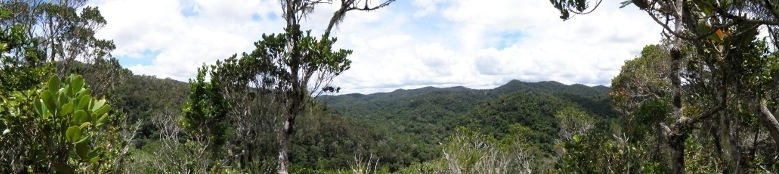
\includegraphics[width=10cm]{figs/Banniere}\\
    \vspace{0.3cm}
    \small{Clément STAHL$^{1}$\hspace{0.25cm}Ghislain VIEILLEDENT$^{2}$\hspace{0.25cm}METRADICA group$^{3}$}\\
    \vspace{0.15cm}
    {\scriptsize
      \begin{tabular}{l}
        $[1]$ \textbf{INRAe} UMR Ecofog, $[2]$ \textbf{Cirad} UMR AMAP, $[3]$ \textbf{METRADICA}
      \end{tabular}
    }\\
    \vspace{0.3cm}
    
\includegraphics[width=0.80\textwidth]{figs/partners_logos}
    
  \end{center}
  \end{frame}
}

% %%%%%%%%%%%%%%%%%%%%%%%%%%%%%%%%%%%%%%%%%%%%%%%%%%%%%%%%%%%%%%%%

\placelogotrue
\begin{frame}
  \frametitle{Plan}
  \begin{columns}[c]
    \begin{column}{0.5\textwidth}
      \tableofcontents[sections=1]
      \vspace{0.5cm}
      \tableofcontents[sections=2]
    \end{column}
    \begin{column}{0.5\textwidth}
        \tableofcontents[sections=3]
        \vspace{0.5cm}
        \tableofcontents[sections=4]
    \end{column}
  \end{columns}
\end{frame}
\placelogofalse

\section{Introduction}
\label{sec:org2358968}

\subsection{Context}
\label{sec:org657aaac}

\begin{frame}[label={sec:orgcb2e860}]{Context}
\begin{itemize}
\item \alert{METRADICA}: Using mechanistic traits to assess tropical forest vulnerability to climate change in French Guiana.
\item 3 years: 01/2020 -- 12/2023.
\item 200,000 euros funded by Labex CEBA.
\item Two PhD (Marion and Jeanne) and one post-doc (Salman).
\item (PhD of Daniela).
\end{itemize}
\end{frame}

\begin{frame}[label={sec:org1ae356f}]{Work during the first two years of the project}
\begin{itemize}
\item Groups have been working separately on the first 3 Tasks of the project: \newline \alert{1.} Data, \alert{2.} Trait x Env, \alert{3.} jSDM, (\alert{4.} Model comp).
\item Field work: 3 missions for the PhD of Marion, 1 mission for the post-doc of Salman.
\item Online meetings (\textasciitilde{} 1/year).
\item We haven't had the chance to meet together yet.
\end{itemize}
\end{frame}

\subsection{Objectives}
\label{sec:orgc485fa3}

\begin{frame}[label={sec:org8ec6813}]{Objectives}
\begin{itemize}
\item Meet in person all together.
\item Present the advances of the different groups.
\item Help students and post-docs advancing their work.
\item Identify tasks that can be done together during this week.
\item Discuss the perspectives and deliverables for each Task.
\end{itemize}
\end{frame}

\subsection{Participants}
\label{sec:org2175d28}

\begin{frame}[label={sec:org7d9040a}]{Participants}
\begin{columns}
\begin{column}{0.5\columnwidth}
\begin{block}{In person}
\begin{itemize}
\item Marion Boisseaux
\item Jeanne Clément
\item Géraldine Derroire
\item Claire Fortunel
\item Vincent Freycon
\item Salman Khan
\item Daniela Krebber
\item Isabelle Maréchaux
\item Heidy Schimann
\item Clément Stahl
\item Ghislain Vieilledent
\end{itemize}
\end{block}
\end{column}

\begin{column}{0.5\columnwidth}
\begin{block}{Remotely}
\begin{itemize}
\item Sabrina Coste
\item Bruno Ferry
\item Gaëlle Jaouen
\end{itemize}
\end{block}
\end{column}
\end{columns}
\end{frame}

\section{Organization}
\label{sec:org5d1adb7}

\subsection{Dates and place}
\label{sec:org8124640}

\begin{frame}[label={sec:orga02092d}]{Dates and place}
\begin{itemize}
\item From 06 to 10 Mars 2023 at AMAP, Montpellier.
\item Morning: 09h00 à 12h30.
\item Afternoon: 14h00 à 17h30.
\item Friday afternoon will be free.
\item We have booked rooms 201 of building PS2 and room 44 of building PS1 (+ office) for work in groups.
\end{itemize}
\end{frame}

\subsection{Meals}
\label{sec:orgeaf9ba2}

\begin{frame}[label={sec:orgf6f0bf3}]{Meals}
\begin{itemize}
\item Lunch at the Cirad cafeteria (12 euros for external people).
\item Reimbursement of mission expenses.
\item Wednesday evening: diner in the city center of Montpellier \newline \(\rightarrow\) booking.
\end{itemize}
\end{frame}

\subsection{Taxis for Tuesday}
\label{sec:orgfd5c751}

\begin{frame}[label={sec:org601f2a6}]{Taxis for Tuesday}
\begin{itemize}
\item Strike on Tuesday 07/03, no public transport.
\item Taxis (Jeanne, Ghislain, Daniela).
\item Meeting at Place Albert 1er (tram station line 1) at 08h30 \newline \(\rightarrow\) booking.
\end{itemize}
\end{frame}

\subsection{Zoom and GoogleDrive}
\label{sec:org879e9dd}

\begin{frame}[label={sec:org7c42870}]{Zoom and GoogleDrive}
\begin{itemize}
\item Zoom: \url{https://umontpellier-fr.zoom.us/j/3624626507}.
\item METRADICA GoogleDrive.
\end{itemize}
\end{frame}

\subsection{Contacts for organization}
\label{sec:org5aba035}

\begin{frame}[label={sec:org9db85c4}]{Contacts for organization}
\begin{itemize}
\item Ghislain Vieilledent, \href{mailto:ghislain.vieilledent@cirad.fr}{ghislain.vieilledent@cirad.fr} \newline tel: 06.24.62.65.07, PS1 bureau 32.
\item Marie-Laure De Guillen, \href{mailto:marie-laure.de\_guillen@cirad.fr}{marie-laure.de\_guillen@cirad.fr} \newline tel: 04.67.61.57.65, PS2 bureau 308.
\end{itemize}
\end{frame}

\section{Agenda}
\label{sec:org4e715cf}

\subsection{Monday and Tuesday}
\label{sec:org244b053}

\begin{frame}[label={sec:org0d6089f}]{Monday}
\begin{block}{Morning}
\begin{itemize}
\item Agenda of the workshop, objectives (Ghislain).
\item Briefly presenting METRADICA and the 4 Tasks (Clément).
\item Budget presentation (Clément and Ghislain).
\end{itemize}
\end{block}

\begin{block}{Afternoon}
\begin{itemize}
\item First results of Marion's PhD, Task 2 (45 min + 45 min of discussion).
\item Break (\textasciitilde{}30 min).
\item First results of Salman's post-doc, Task 1 on soils (45 min + 45 min of discussion).
\end{itemize}
\end{block}
\end{frame}

\begin{frame}[label={sec:org5464612},fragile]{Tuesday}
 \begin{block}{Morning}
\begin{itemize}
\item First results of Jeanne's PhD (30 min + 30 min discussion).
\item Presenting the \texttt{gecevar} R package for getting climatic and environnemental variables (30 min).
\item Tutorial on the use of \texttt{gecevar} and \texttt{jSDM} (1h30).
\end{itemize}
\end{block}

\begin{block}{Afternoon}
\begin{itemize}
\item Presenting the data-sets (inventories, traits, environnement).
\item Discussing the possibility of a data paper on traits.
\item Organising working groups for the week.
\item Setting objectives for the week (e.g. writing sections of articles, tables, figures, data analysis, map making, data-set building, etc.).
\end{itemize}
\end{block}
\end{frame}

\subsection{Wednesday and Thursday}
\label{sec:orgd34a03a}

\begin{frame}[label={sec:org0049491}]{Wednesday and Thursday}
\begin{block}{Morning}
\begin{itemize}
\item Working by group.
\end{itemize}
\end{block}
\begin{block}{Afternoon}
\begin{itemize}
\item Working by group.
\item Summary of working group advances.
\end{itemize}
\end{block}
\end{frame}

\subsection{Friday}
\label{sec:org99b291f}

\begin{frame}[label={sec:org8e439e6}]{Friday}
\begin{block}{Morning}
\begin{itemize}
\item Working by group.
\item List of planned articles with title, persons involved, and deadlines.
\item Discussion on perspectives, new projects, or link with current projects (ALT, ANR, FEDER, PEPR Forest, CEBA3).
\end{itemize}
\end{block}
\end{frame}

% %%%%%%%%%%%%%%%%%%%%%%%%%%%%%%%%%%%%%%%%%%%%%%%%%%%%%%%%%%

{
  % Use background image
  \usebackgroundtemplate{%
    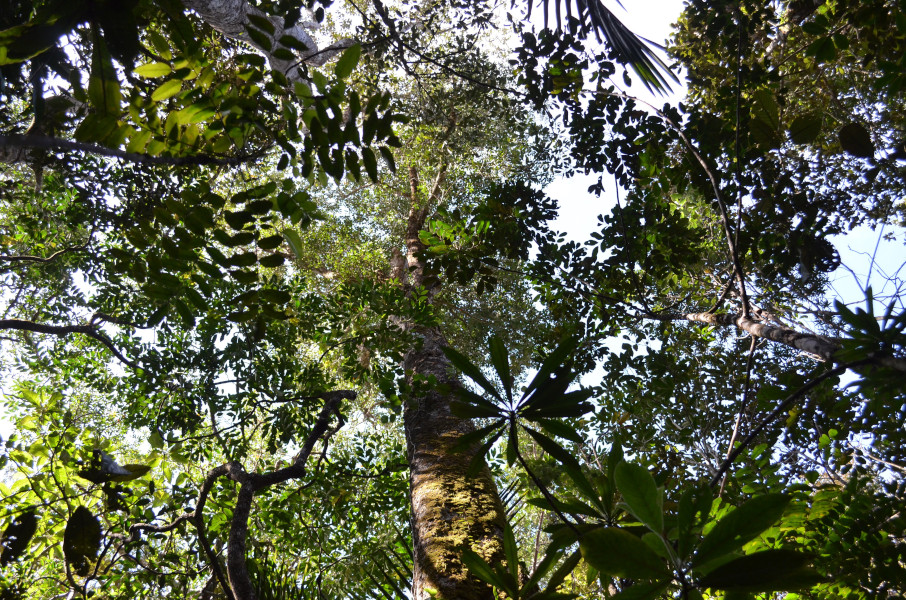
\includegraphics[keepaspectratio=true, height=\paperheight]{figs/Canopy-NC}
  }
  \setbeamertemplate{navigation symbols}{}
  % Remove shadow from block
  \setbeamertemplate{blocks}[rounded][shadow=false]
  \begin{frame}[plain]
  	\vspace*{\stretch{100}} 
    \begin{block}{}
      \begin{center}
        \ldots~Thank you for attention~\ldots \\
        \url{https://ecology.ghislainv.fr/presentations} \\
        
\includegraphics[width=0.55\textwidth]{figs/partners_logos}
      \end{center}
    \end{block}
  \end{frame}
}
\end{document}